\section{Algorithms \& System Model}
\noindent Unlike traditional centralized localization systems that rely on raw trilateration, this project's proposed solution, namely "ICUM" system, implements a distributed state machine where node roles are dynamic and position estimation is performed via a cooperative graph optimization algorithm.

\subsection{Dynamic Role Management}
\noindent The network operates as a Destination-Oriented Directed Acyclic Graph (DODAG) for sending messages. Nodes autonomously switch between roles based on their connectivity state and sensor readings. Let $R_i(t)$ denote the role of the node $i$ at time $t$. The state space is defined as: 
\begin{equation}
    R \in \{ROOT, LEADER, RELAY, IDLE, ISOLATED\}
\end{equation}
A node in the state $IDLE$ must send its messages "up" to either $RELAY$s or $LEADER$s, hence why the messaging strategy is based on DODAG. Transitions are governed by the tuple ($H_{gw}, N{neighbors},T_{iso}$), where $H_{gw}$ is the hop count to a gateway, $N_{neighbors} = 0$ for a duration $t > T_{iso}$. A node promotes itself to $R = LEADER$ if it wins the local election process defined in section 3.4.

\subsection{Hardware}
\noindent Since every node needs the capabilities to fill whatever role the system requires at any given state, the hardware stack must be homogeneous. Below is a tentative hardware specification that fulfils all the requirements of the system:
\begin{itemize}
    \item \textbf{Computation}: MCU (e.g., Nordic nRF52/53 or STM32)
    \item \textbf{Sensors}: 6-axis IMU (Accelerometer/Gyro)
    \item \textbf{Communication}: BLE for Mesh data \& Signalling
    \item \textbf{Ranging}: UWB (DW3000) for TWR Distance \& AoA
    \item \textbf{Backhaul}: LTE-M / NB-IoT
\end{itemize}
MCUs are ideal for distributed systems \cite{MicrocontrollerUnit-BasedWirelessSensorNetworkNodes:AReview}, given their low latency, ultra-low power consumption, and durability in systems that never shut down. As for the inertial movement detector, any low-power accelerometer can be used, but IMU sensors have been chosen for their accuracy and potential for self-optimization based on inertial movement. The communication strategy will revolve around many instances of one-to-one communication, making BLE an effective option for sending and receiving messages. Note that over large distances, BLE can experience significantly reduced effectiveness, so this choice may need reconsidering depending on the application domain. As mentioned before, UWB will be used for ranging, and if a node is unable to detect any $LEADERS$ or $RELAYS$, it will use LTE-M, which is effective in low-power areas, to detect its own location with GPS as well as possible. Naturally, this goes against the design philosophy and intended application of the system, but it is only used as a backup option for when no other location detection or computation is available.

\subsection{States and Communication}
\noindent The states related to the movement of the wireless sensor nodes are depicted below in figure \ref{fig:states}. When a node joins the network, the initial internal state is $STATIONARY$, even if the node itself is physically moving. When its inertial sensor is turned on, it will start to monitor its movement, and if it exceeds $0.5G$, it will transition to the $MOVING$ state. While moving, it will turn off its relay properties, preventing it from forwarding messages from neighbouring nodes to $LEADERS$. Moving nodes are naturally volatile, making their relay capabilities more unreliable and unstable, which is the basis for this design choice. While moving, nodes will repeatedly perform UWB blinking to receive location information from the neighbouring nodes. A neighbouring node that responds to UWB ranging must send an acknowledgment to ensure that the UWB blinking was noticed by at least one neighbouring node. If a $MOVING$ node has not received acknowledgements for 30 seconds, or a $STATIONARY$ node has not detected UWB blinking for 30 seconds, it will transition to the $ISOLATED$ state. In this state, the node will continuously scan for nearby mesh networks in an attempt to join a cluster, and without the possibility for cooperative localization, it will fall back to GPS despite potentially being in a GPS-denied environment. The location will be transmitted to the cloud regardless of accuracy, and if a mesh network is found, depending on the movement of the node, it will either transition back to $STATIONARY$ or $MOVING$.\\

\noindent Illustrated in figure \ref{fig:sequence} is a sequence diagram modelling the communication between the different nodes and cloud service. The $Moving\  Tracker$ object will initiate communication by sending a message to any $Neighbouring\ Nodes$ to which they will respond by measure the AoA and euclidean distance from themselves to the messaging node. They will follow up with an acknowledgment and the location information that the $Moving\ Tracker$ will use to update its internal location. This will then be sent to the nearest $Leader$ node, and forwarded to the $Cloud$. if the $Moving\ Tracker$ is in the $ISOLATED$ state, it will send its own GPS location directly to the $Cloud$, however inaccurate it may be. 

\begin{figure*}[t] %float with two figures
\centering
\includegraphics[width= 1\linewidth]{images'nshi/stateDiagram.png}
\caption{State diagram of the wireless sensor nodes depicting the relation between states and transitions\label{fig:states}}\bigskip 
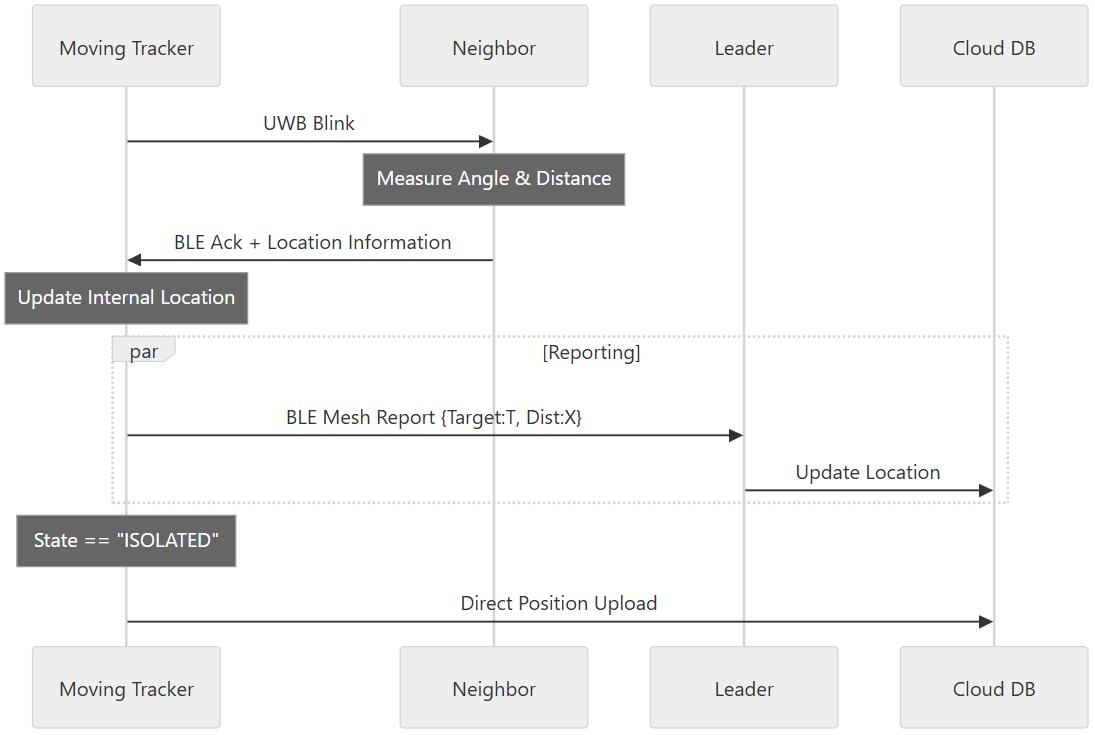
\includegraphics[width= 1\linewidth]{images'nshi/Seq.png}
\caption{Sequence Diagram illustrating message interaction between Moving Trackers, Neighbouring nodes, Leaders, and the Cloud\label{fig:sequence}}
\end{figure*}
%\begin{figure*}[h]
    %\centering
    %\includegraphics[width=1\linewidth]{images'nshi/stateDiagram.png}
    %\caption{State diagram of the wireless sensor nodes depicting the relation between states and transitions}
 %   \label{fig:states}
%\end{figure*}

%\begin{figure*}[h]
 %   \centering
  %  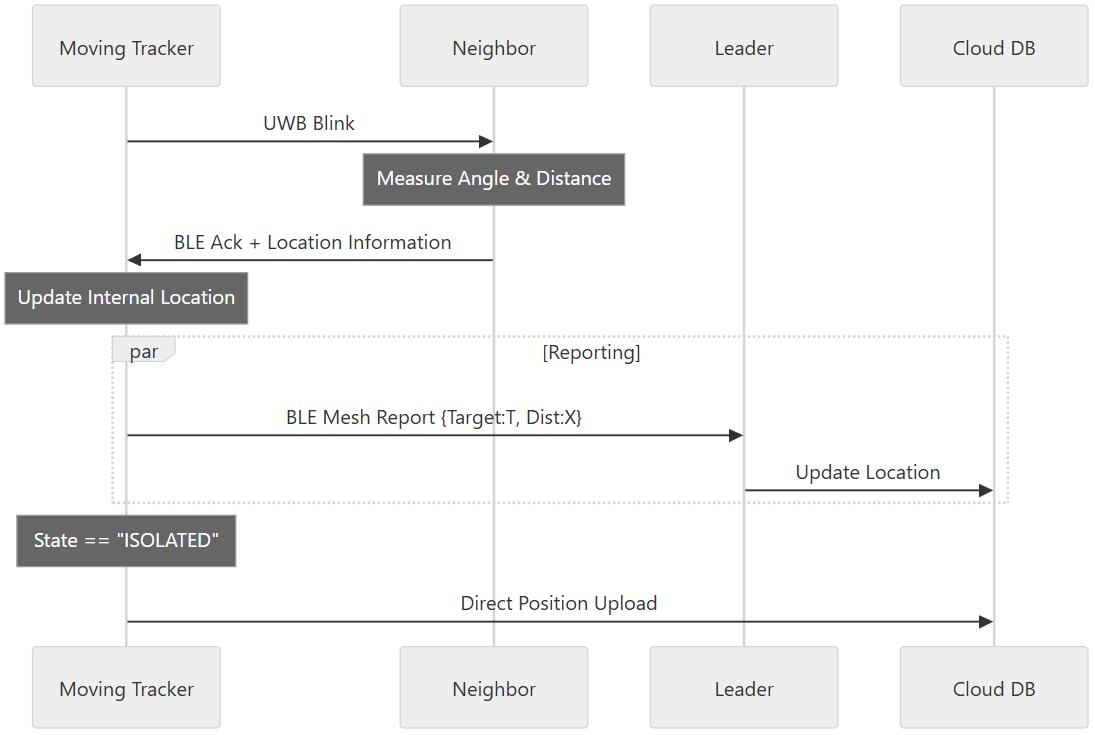
\includegraphics[width=1\linewidth]{images'nshi/Seq.png}
   % \caption{State diagram of the wireless sensor nodes depicting the relation between states and transitions}
    %\label{fig:sequence}
%\end{figure*}


\subsection{Battery-Aware Consensus Protocol}
\noindent To ensure network longevity, cluster $LEADERS$ are not chosen randomly but through a deterministic, battery-aware variation of the Bully Algorithm. The system implements a multi-criteria decision function $f(n)$ to rank candidate nodes. For a set of candidates nodes $C$ (local neighbours $\cup \space self$), the optimal leader $L$ is selected as: 
\begin{equation}
    L = argmax_{n \in C} (P_{hw}(n), N_{deg}(n), B(n), ID(n))
\end{equation}
Where the priority hierarchy is defined as:
\begin{itemize}
    \item \textbf{Hardware Capability ($P{hw}$):} Nodes with active LTE backhaul ($H_{gw} < 100$) are prioritized strictly over battery-powered nodes.
    \item \textbf{Degree Centrality ($N_{deg}$:} Nodes with a higher neighbour count are preferred to maximize mesh coverage.
    \item \textbf{Residual Energy ($B$):} Among nodes with equal connectivity, the node with the higher battery $B(n)$ is selected.
    \item \textbf{Tie-Breaker ($ID$):} Lower node IDs break ties to ensure deterministic convergence.
\end{itemize}
This modification prevents the same election spiral that is common in standard bully algorithms, where a dying node keeps re-electing itself simply because it has the highest ID.


%maybe COMPARE WITH EXISINTG LEADER ELECTION ALGOS, ANALYZE HOW GOOD IT IS, HOW MANY OPERATIONS WILL IT TAKE WITH 'n' nodes to find a leader?

\subsection{Distributed Graph Optimization}
\noindent The core localization engine utilizes a force-directed graph approach known as spring relaxation rather than algebraic trilateration. This allows the system to be resilient to noise and recover from temporary non-line-of-sight (NLOS) conditions. The network is modelled as a graph $G = (V, E)$, where $V$ represents nodes and $E$ represents UWB ranging constraints. The state of node $i$ is its position vector \textbf{$P_i = [x_i, y_1]^T$} and orientation \textbf{$\theta_i$}. The objective is to minimize the global cost function \textbf{J}:
\begin{equation}
    J = \sum_{(i,j) \in E} (\lambda_d * e_{dist}(i,j)^2 + \lambda_\theta * e_{angle}(i,j)^2)
\end{equation}
where $\lambda_d$ and $\lambda_\theta$ are weights denoted as learning rates for distance and angular constraints, respectively.

\noindent For a measured UWB range $d_{ij}$ between node $i$ and $j$, the error term is the difference between the measured range and the Euclidean distance of the current estimates:
\begin{equation}
    e_{dist}(i,j) = || P_j - P_i || - d_{ij}
\end{equation}
The correction vector $\Delta\bf{P}_{dist}$ applied to node $i$ is derived from the gradient where $\alpha$ is the learning rate (configured to 0.2 in the implementation):
\begin{equation}
    \Delta\bf{P}_{dist} = \alpha * e_{dist}(i,j) * \frac{P_j - P_i}{|| P_j - P_i ||}
\end{equation}
